\chapter{Experiment}

To analyze the properties of a ring resonator, a scaled microwave model is used. The setup is shown in Figure \ref{fig:setup}\footnote[1]{Jingshi Li, Materials for the preparation of Experiment 6}. The transmission through this waveguide structure (|$S_{21}$|) is analyzed with a network analyser (NWA). For each measurement the NWA was calibrated without the resonator 
\begin{figure}%
\centering
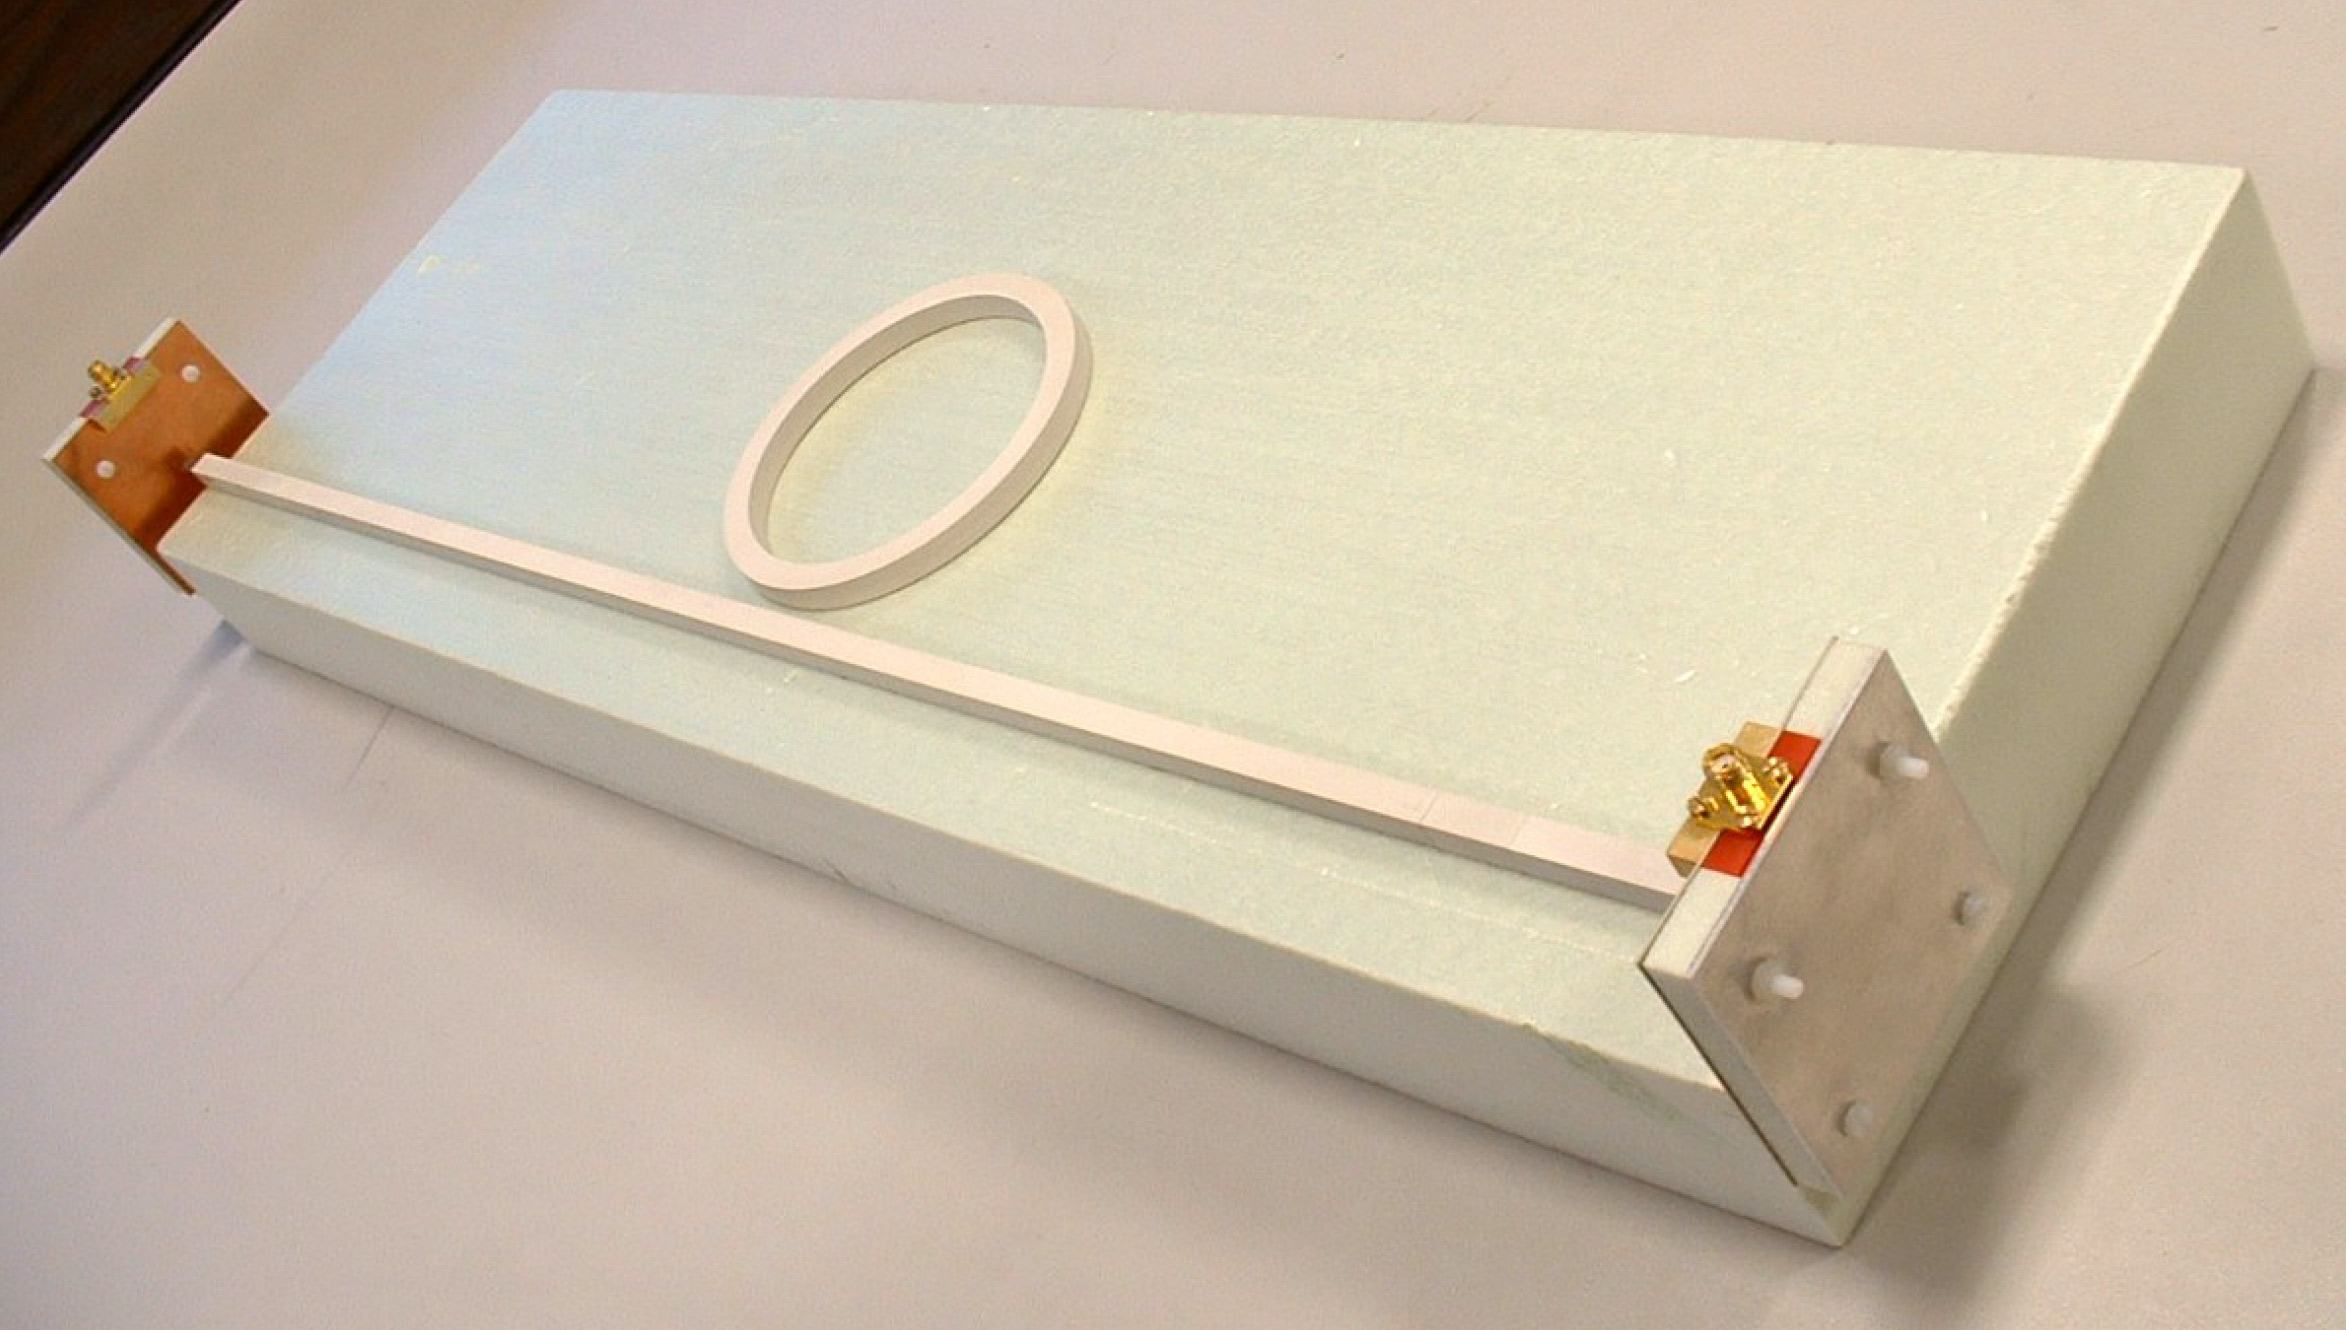
\includegraphics[width=.5\columnwidth]{Grafiken/foto_resonator.jpg}%
\caption{Experimental Setup}%
\label{fig:setup}%
\end{figure}

\section{Influence of the distance of the ring}
First a ring with a radius of $r_1$~=~22.6~mm was analyzed. Therefore frequencies between 8 and 10.8~GHz were measuered with 1601 points. The transmission through the setup without any ring resonator was measured and subtracted out with the calibration of the NWA.

The ring was set in direct contact to the line. The transmission changed immediatly. At certain frequencies the transmission breaks in and characteristic dips of the ring resonator can be observed. Figure \ref{fig:01_s21} shows the transmission $|S_{21}|$ through the setup for different distances between the ring and the transmission line.
For lager distance the dips become less deep and the resonance frequency shifts to lower frequencies. The coupling into the ring resonator becomes weaker for higher distances.
 
\begin{figure}%
\centering
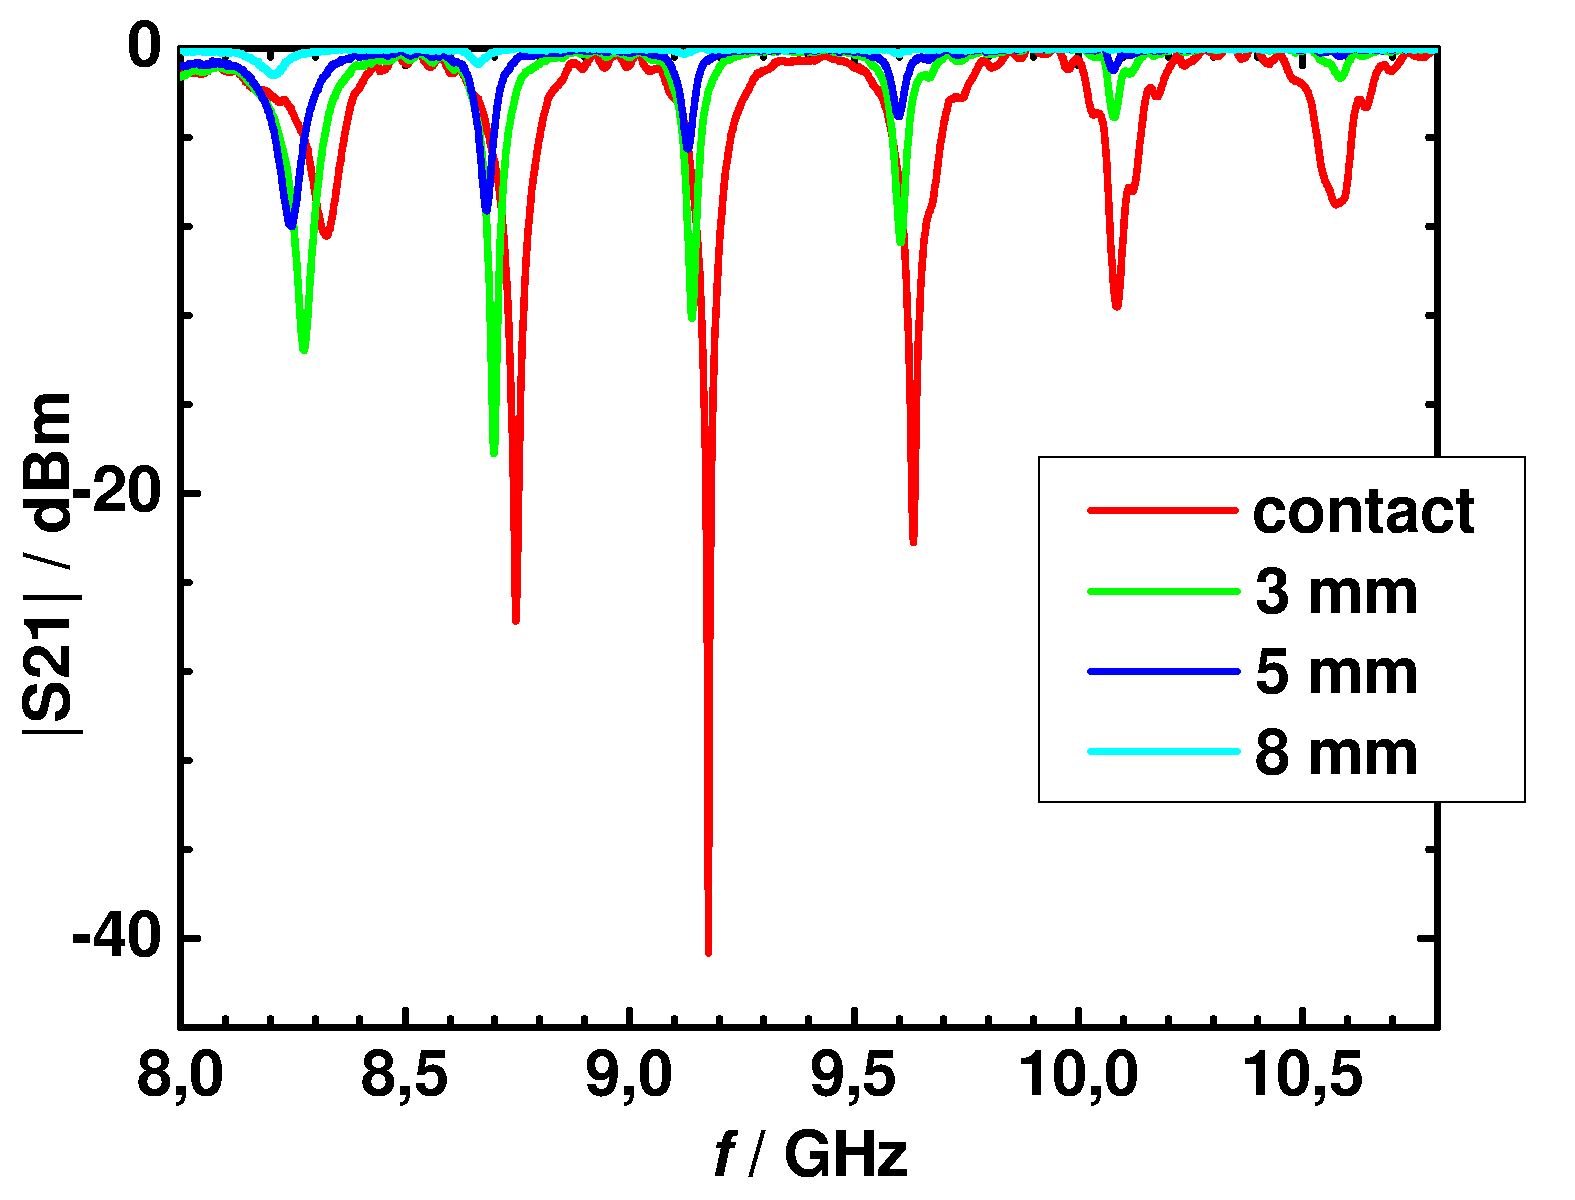
\includegraphics[width=.6\columnwidth]{Grafiken/01_s21.pdf}%
\caption{|$S_{21}$| for different distances between the transmission line and the ring resonator ($r_1$~=~22.6~mm).}%
\label{fig:01_s21}%
\end{figure}

Between a distance of 0~mm and 1~mm the dips become deepest, the transmission gets minimal. In this area there is the case of critical coupling. 

To analyze this the frequency range was changed to 9~GHz~-~9.8~GHz. In this range two dips can be observed. By changing the distance between the ring resonator and the transmission line the minimal transmission at the resonance frequencies was minimized. It was not possible to get both dips below -40~dB. The best result was achieved for a distance of $\sim$0.75~mm. Figure \ref{fig:03_075} shows the transmission for that case.
For this distance $|S_{21}|$(9.16~GHz)~=~-38.3~dB and  $|S_{21}|$(9.62~GHz)~=~-40.3~dB.

$\delta f$ and $\Delta f$ can be extracted from the measurement are given in table \ref{tab:ring_klein}. To read out $\delta f$ the broadness of the dip at |$S_{21}$|~=~-3~dB is measured. \todo{Problem: Dip2 ist oben etwas komisch}
Using equations \eqref{eq:kappa} and \eqref{eq:alpha} $\kappa$ and $\alpha$ can be calculated.
\begin{equation}
\begin{split}
\kappa(9.16~\mathrm{GHz})=0.44\\
\kappa(9.62~\mathrm{GHz})=0.50
\end{split}
\label{eq:}
\end{equation}
\begin{equation}
\begin{split}
\alpha(9.16~\mathrm{GHz})=4.08~\mathrm{m}^{-1}\\
\alpha(9.62~\mathrm{GHz})=4.85~\mathrm{m}^{-1}
\end{split}
\label{eq:}
\end{equation}
\todo{Nochmal nachrechnen, vorallem alpha, da hab ich mehrfach unterschiedliches raus Oo}
The calculated values for both the resonances are quite different. The transmission above the resonance at 9.62~GHz is uneven. Because of this maybe the $\delta f$ is not good enough to measure. 
\begin{table}%
\centering
\caption{Ring resonator ($r_1$~=~22.6~mm) at critical coupling ($d \approx 0.75$~mm). Transmission properties.}
\begin{tabular}{cccccc}
\toprule
$f\i{res}$	& $\delta f$	& $\Delta f$ & $F$ & $\kappa$ & $\alpha$\\
\midrule
9.16 GHz	& 0,086~GHz	& 0.46~GHz	&	5.35&	0.44 & 4.08~m$^{-1}$\\
9.62 GHz	& 0,103~GHz	& 0.46~GHz	&	4.47	&	0.50 & 4.85~m$^{-1}$\\
\bottomrule 
\end{tabular}
\label{tab:ring_klein}
\end{table}



\begin{figure}%
\centering
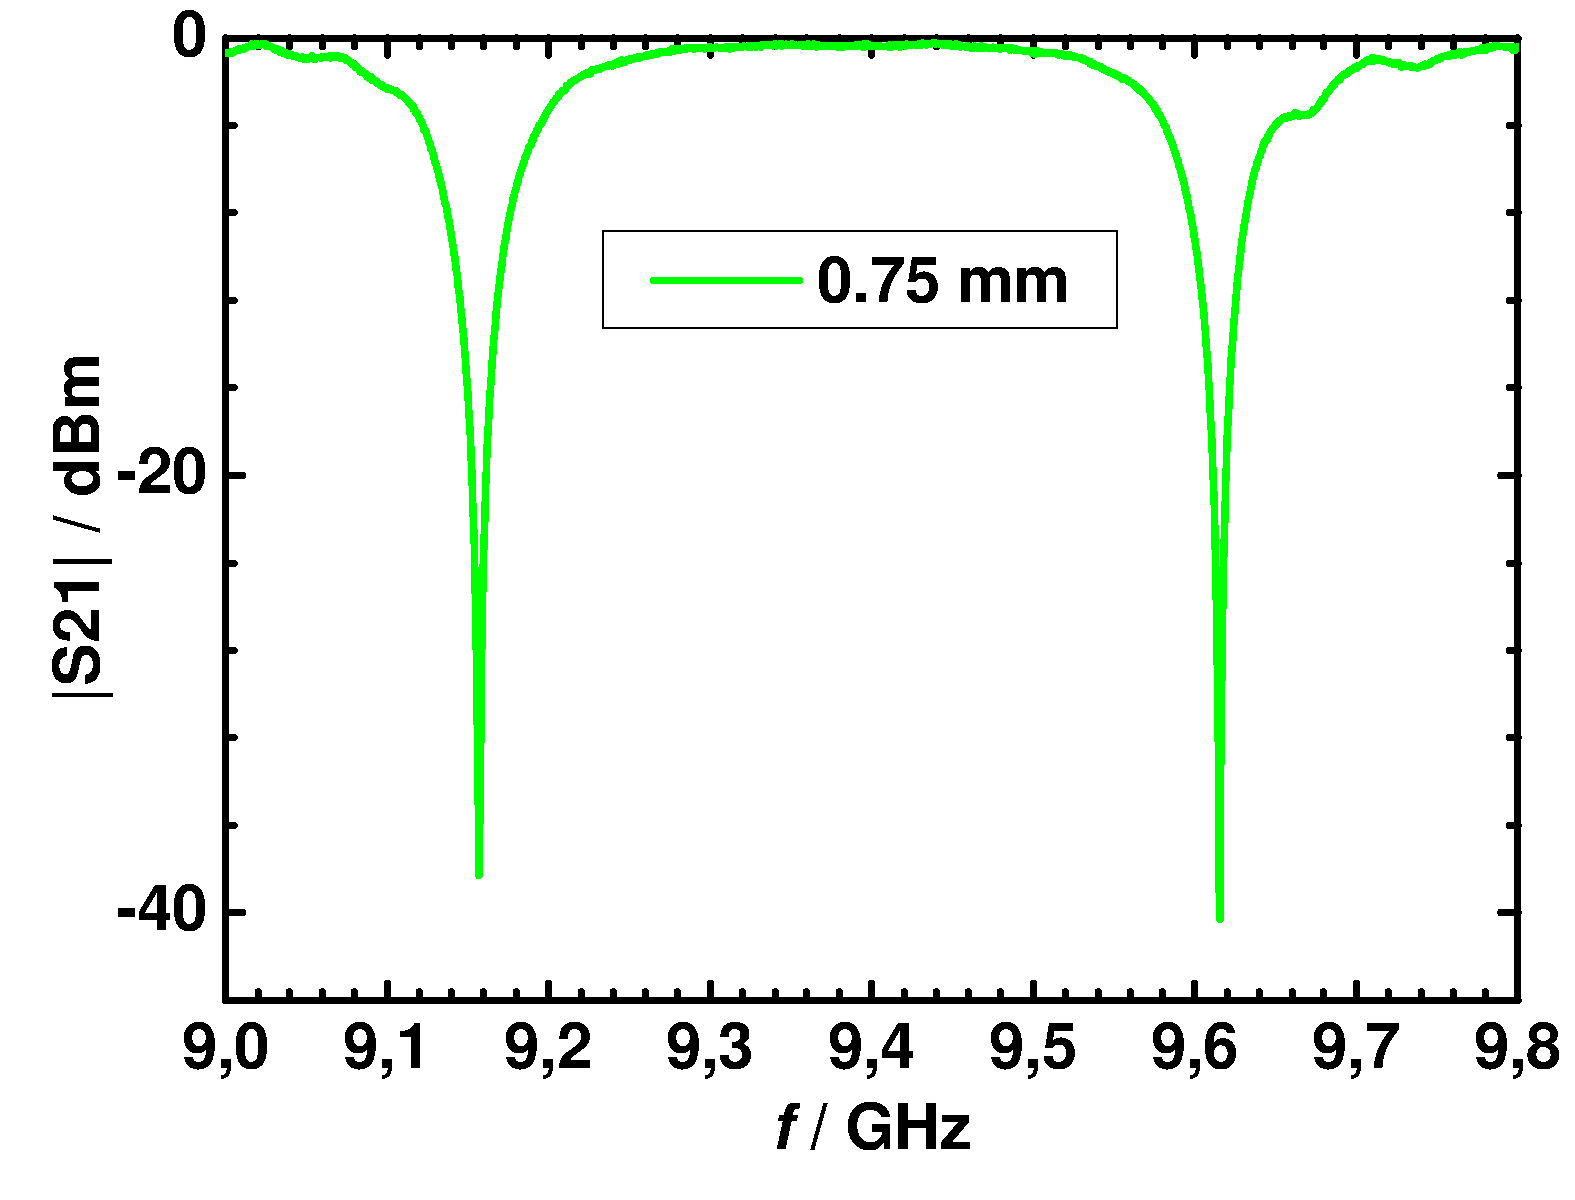
\includegraphics[width=.6\columnwidth]{Grafiken/03_075.pdf}%
\caption{Transmission near the case of critical coupling for a small ring ($r_1$~=~22.6~mm)}%
\label{fig:03_075}%
\end{figure}

Secondly a larger ring with a radius of $r_2$~=~45.1~mm was examined. Comparing the small and the large ring (cf. fig. \ref{fig:04_vergleich}) the large ring shows in the same frequency range twice as much resonances compared to the small ring. This agrees with equation \eqref{eq:abstand} since the  radius of the resonator and therefore length of the resonator has doubled thus the distance between two resonances $\Delta f$ halves.
\begin{figure}%
\centering
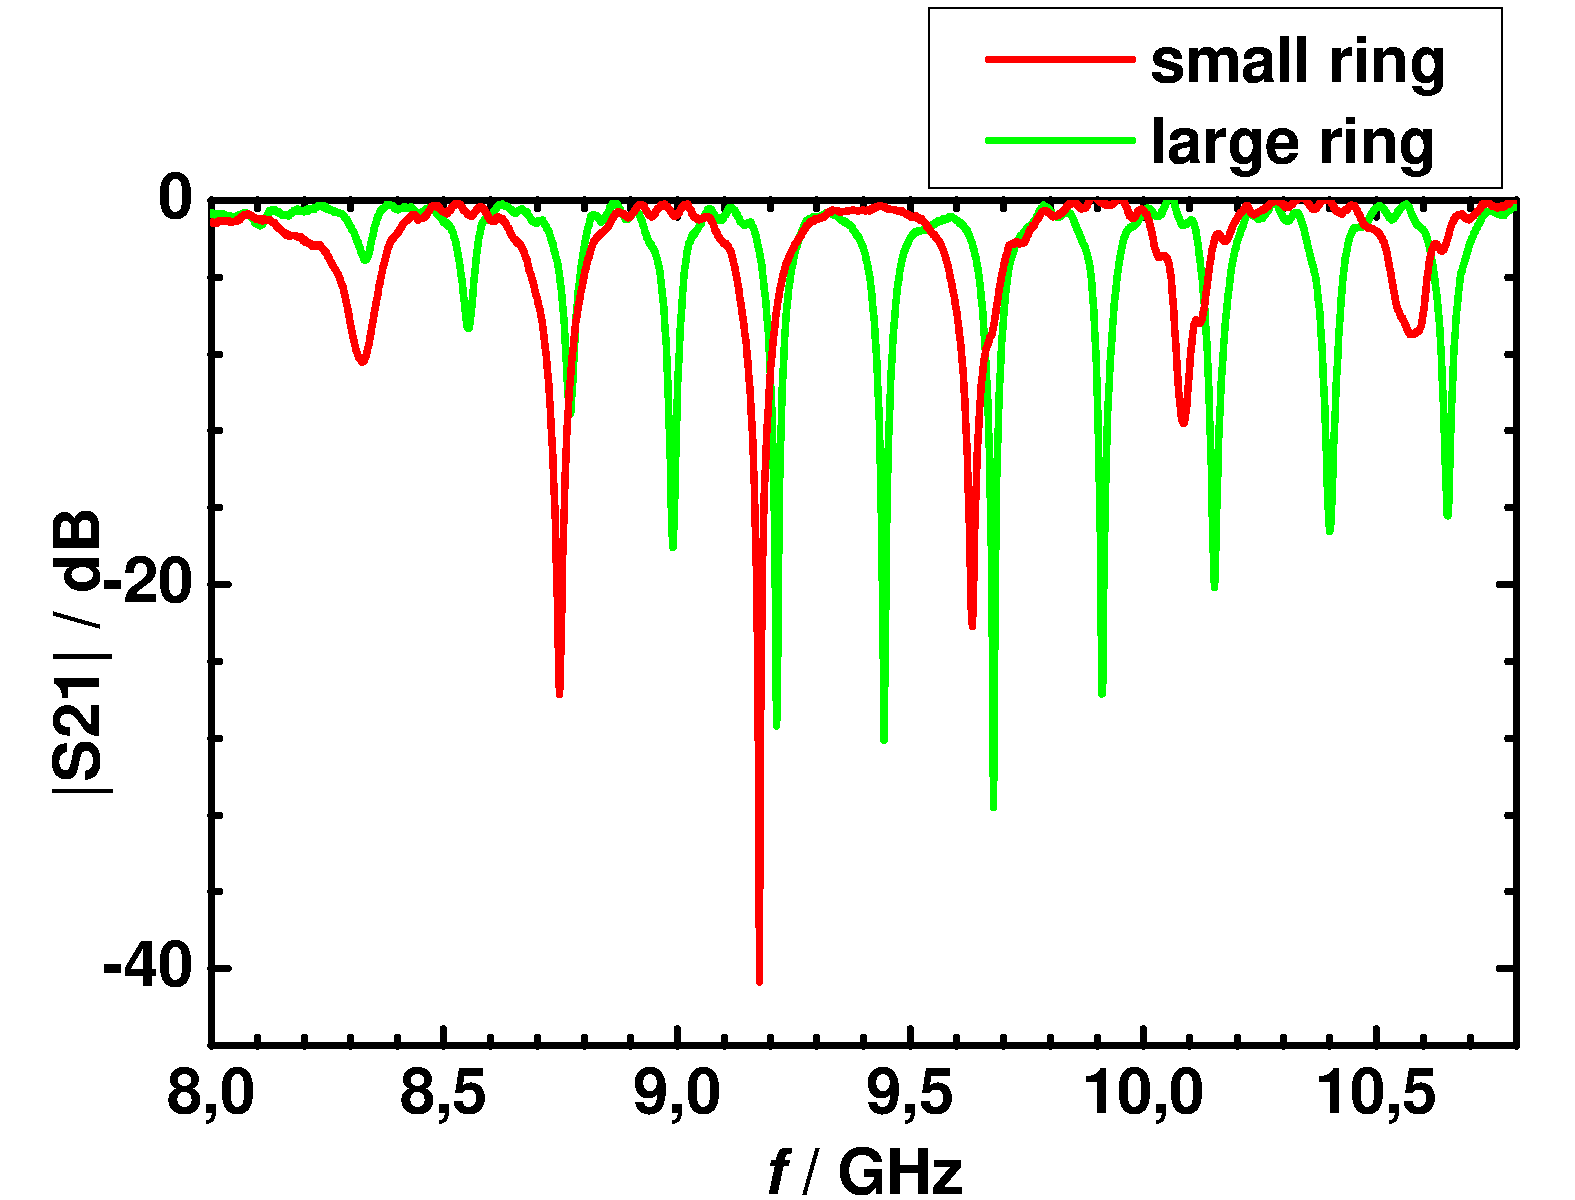
\includegraphics[width=.6\columnwidth]{Grafiken/04_vergleich.pdf}%
\caption{Transmission of the small ring ($r_1$~=~22.6~mm) resonator and a large ring ($r_2$~=~25.1~mm)  resonator.}%
\label{fig:04_vergleich}%
\end{figure}

\begin{table}%
\centering
\caption{Ring resonator ($r_2$~=~45.1~mm) at critical coupling ($d \approx 1.1$~mm). Transmission properties.}
\begin{tabular}{cccccc}
\toprule
$f\i{res}$	& $\delta f$	& $\Delta f$ & $F$ & $\kappa$ & $\alpha$\\
\midrule
9.19 GHz	& 0.057~GHz	& 0.23~GHz	& 4,04	& 0.53	& 2.68~m$^{-1}$ \\
9.42~GHz	&	0.064~GHz	&	0.23~GHz	& 3,59	& 0.57	&	3.00~m$^{-1}$\\
9.66 GHz	& 0,058~GHz	& 0.23~GHz	&	3,97	&	0.54	& 2.72~m$^{-1}$ \\
\bottomrule 
\end{tabular}
\label{tab:ring_gross}
\end{table}

\begin{figure}%
\centering
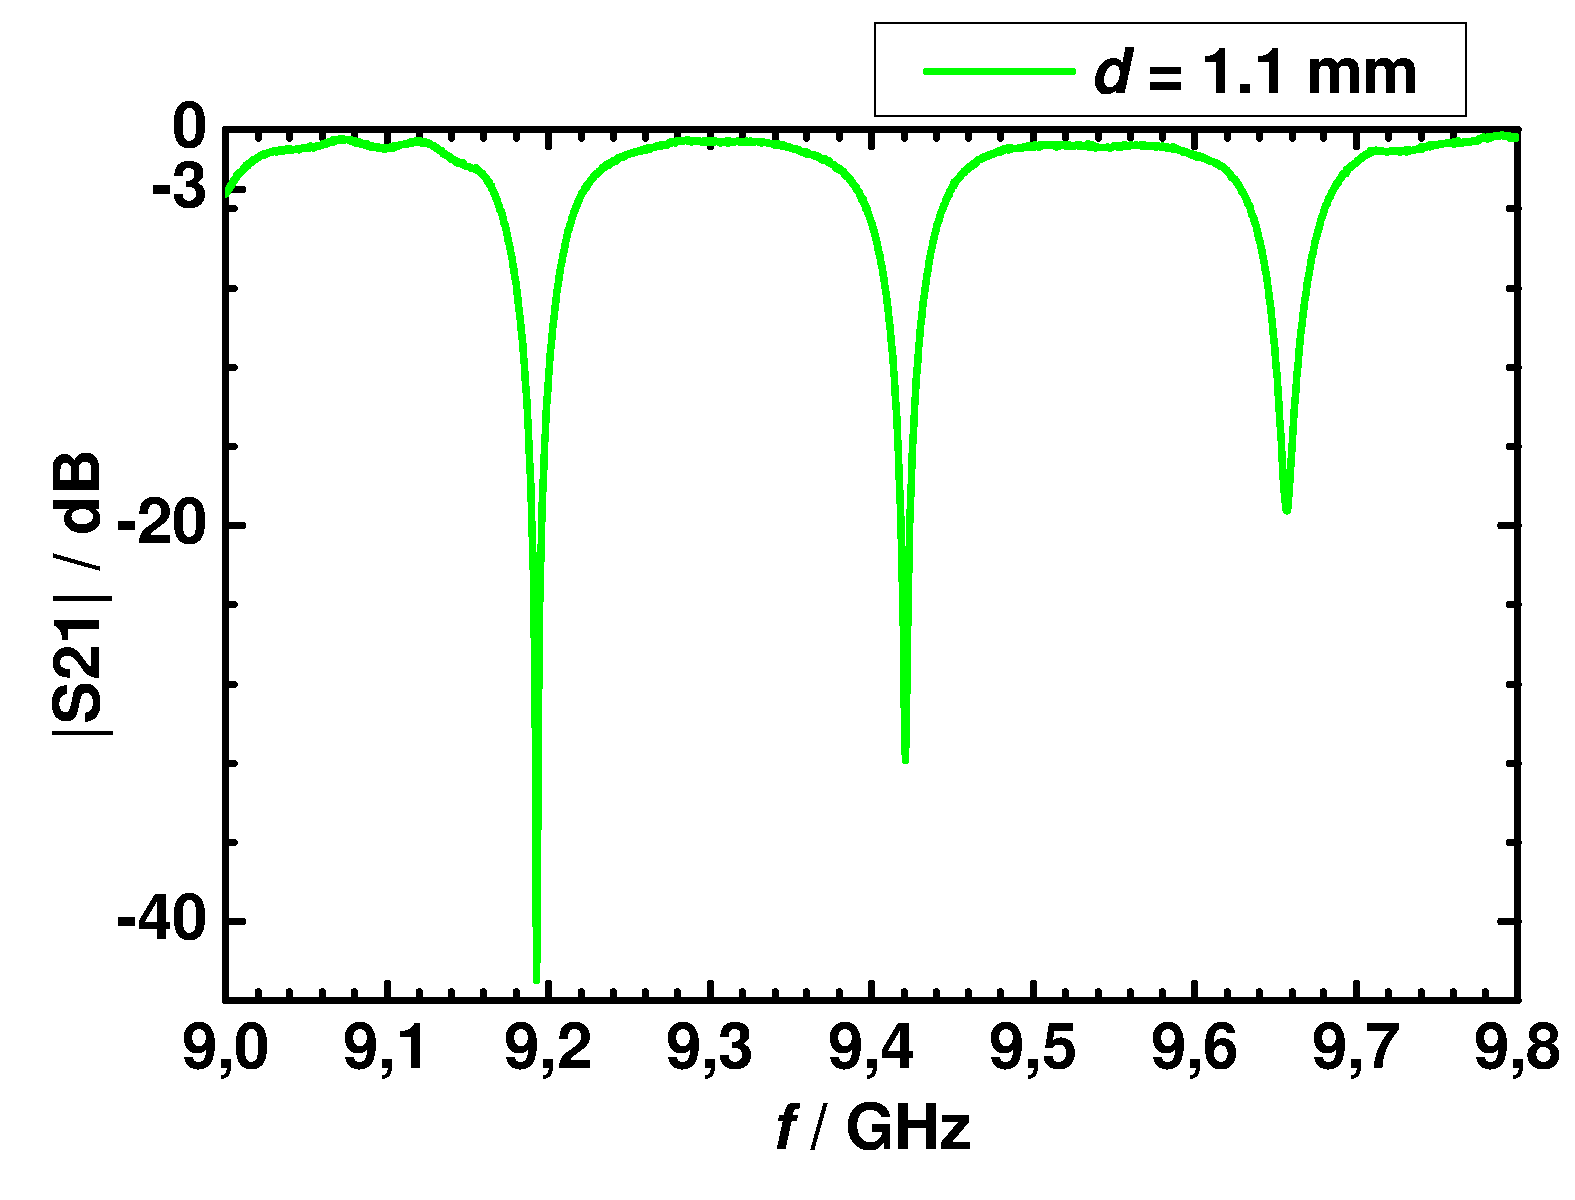
\includegraphics[width=.6\columnwidth]{Grafiken/05_11.pdf}%
\caption{Transmission near the case of critical coupling for a large ring ($r_2$~=~45.1~mm)}%
\label{fig:05_11}%
\end{figure}
Again the distance between the ring and the transmission line was varied to get the lowest transmission at the resonances. \\The best result was achieved at a distance of $\sim$1.1~mm. Here the transmission of at least one resonance is below \mbox{-40~dB}.
The measured transmissions at $d \approx 1.1$~mm are |$S_{21}$|(9.19~GHz)~=~\mbox{-43.0~dB}, |$S_{21}$|(9.42~GHz)~=~\mbox{-32.9~dB} and |$S_{21}$|(9.66~GHz)~=~-19.3~dB.

Assuming that this is the case of critical coupling the coupling coefficient $\kappa$ and the attenuation $\alpha$ can be calculated as before. The values used to calculate are given in table \ref{tab:ring_gross}.
\begin{equation}
\begin{split}
\kappa(9.19~\mathrm{GHz})=0.53\\
\kappa(9.42~\mathrm{GHz})=0.57\\
\kappa(9.66~\mathrm{GHz})=0.54\\
\end{split}
\label{eq:}
\end{equation}
\begin{equation}
\begin{split}
\alpha(9.19~\mathrm{GHz})=2.68~\mathrm{m}^{-1}\\
\alpha(9.42~\mathrm{GHz})=3.00~\mathrm{m}^{-1}\\
\alpha(9.66~\mathrm{GHz})=2.72~\mathrm{m}^{-1}
\end{split}
\label{eq:}
\end{equation}
\todo{Nochmal nachrechnen, vorallem alpha, da hab ich mehrfach unterschiedliches raus Oo}

\todo{compare  the results with the small ring}

The next task was to analyze the group delay change when varying the distance of the ring. Therefore the format of the NWA display was changed to $gruop~delay$. The frequency range was defined as 8.55-9.85~GHz.

\begin{figure}%
\centering
%\begin{adjustwidth}{0cm}{0cm}
%	\subfloat[contact]{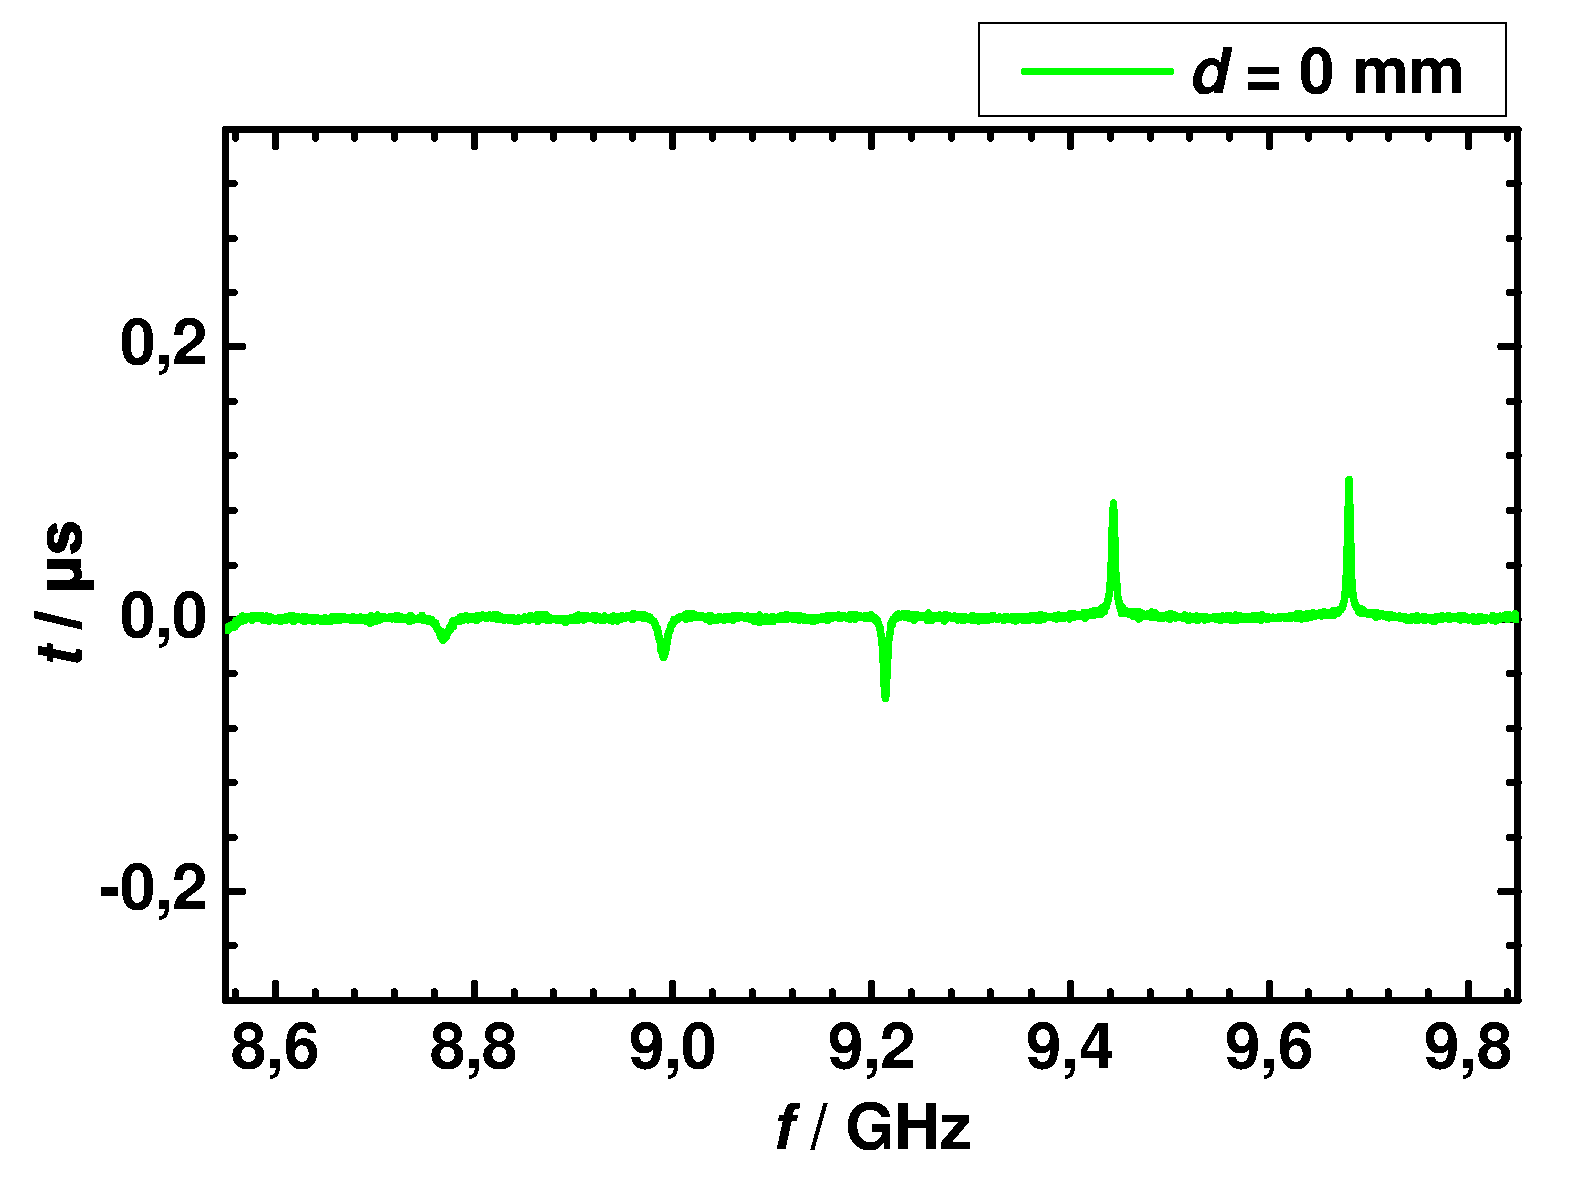
\includegraphics[totalheight=6 cm]{Grafiken/06_0.pdf}\label{fig:06_0}}
	\subfloat[$d = 0.7$~mm]{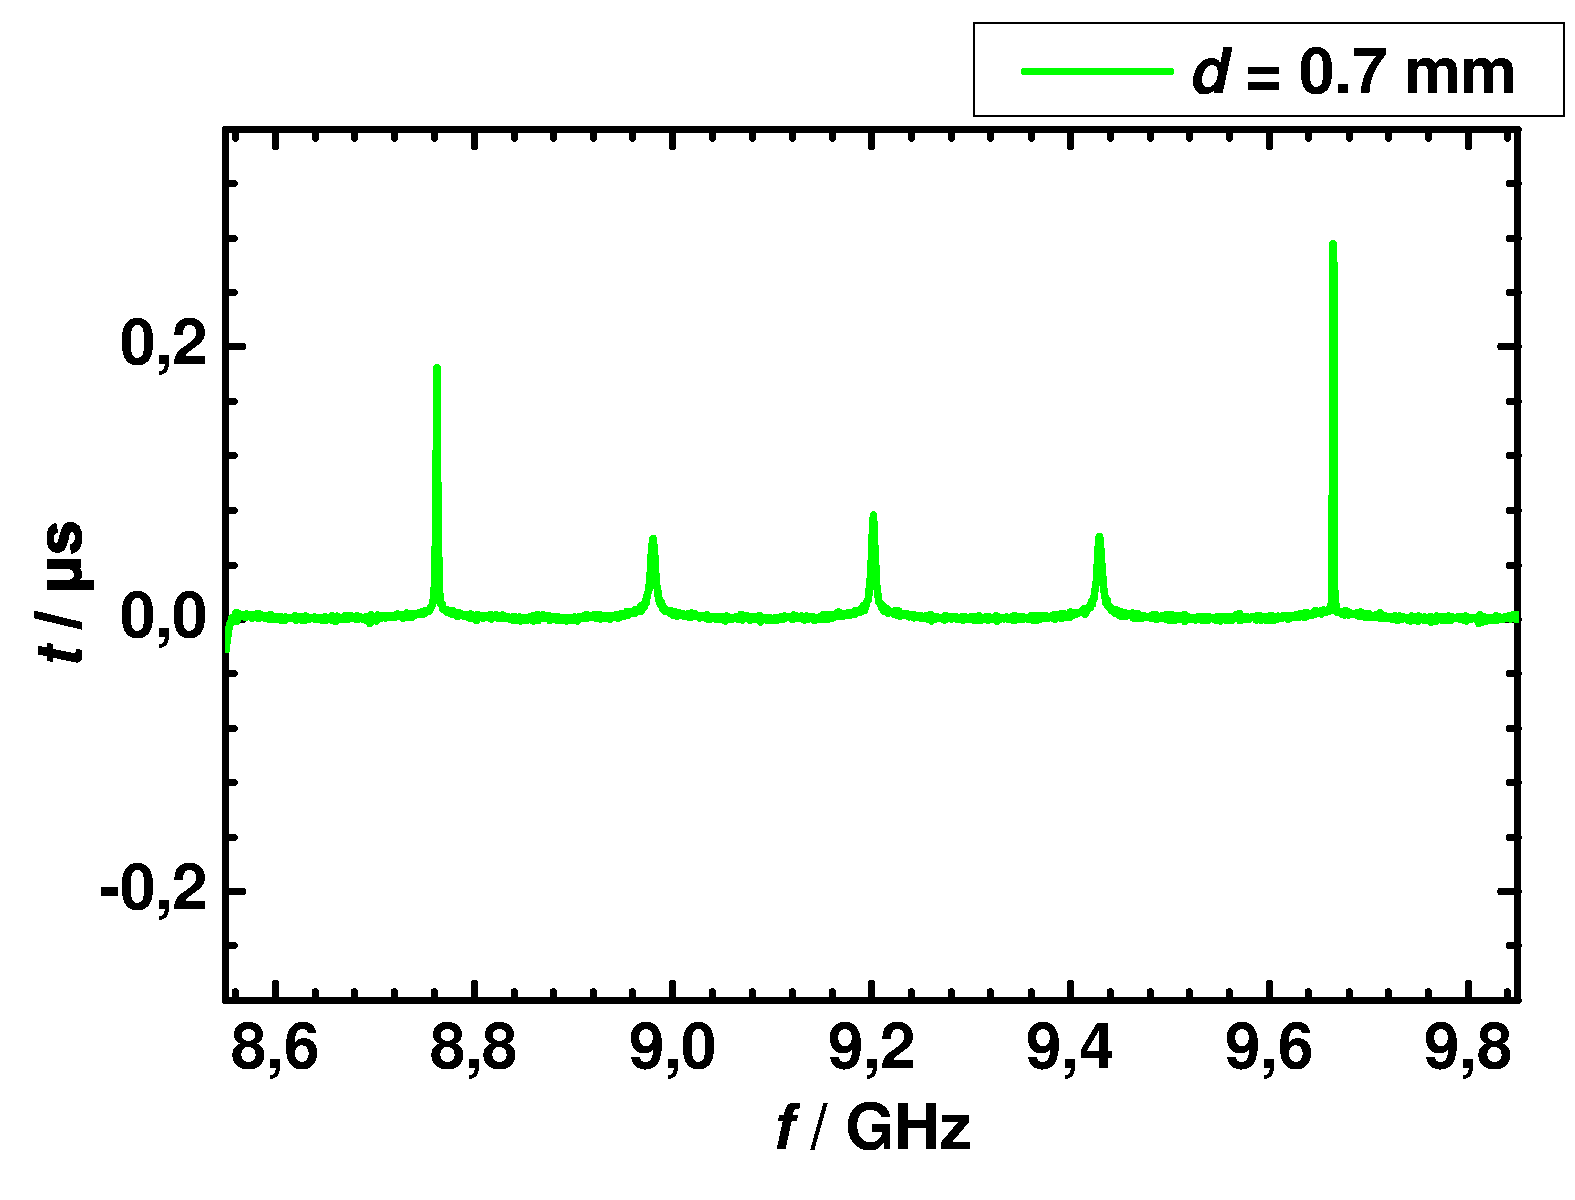
\includegraphics[totalheight=6 cm]{Grafiken/06_07.pdf} \label{fig:06_07}}
		\subfloat[$d = 1.2$~mm]{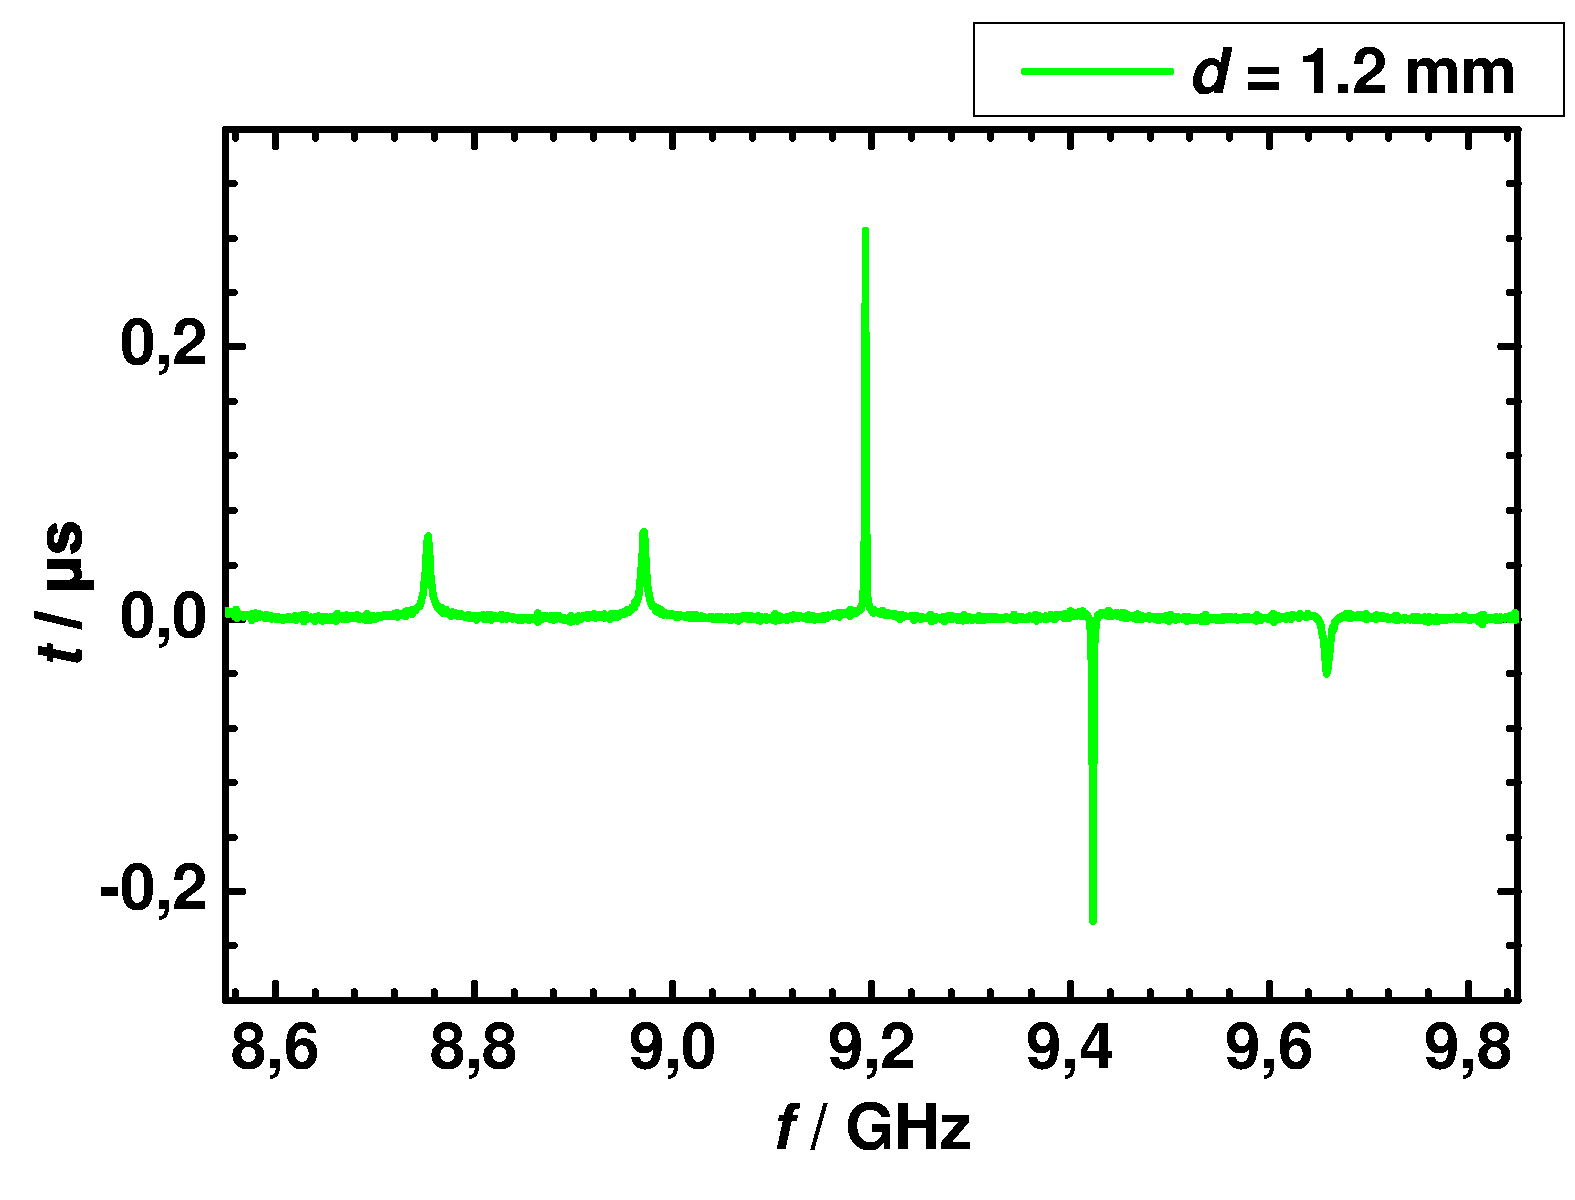
\includegraphics[totalheight=6 cm]{Grafiken/06_12.pdf}\label{fig:06_12}}\\
	\subfloat[$d = 2.2$~mm]{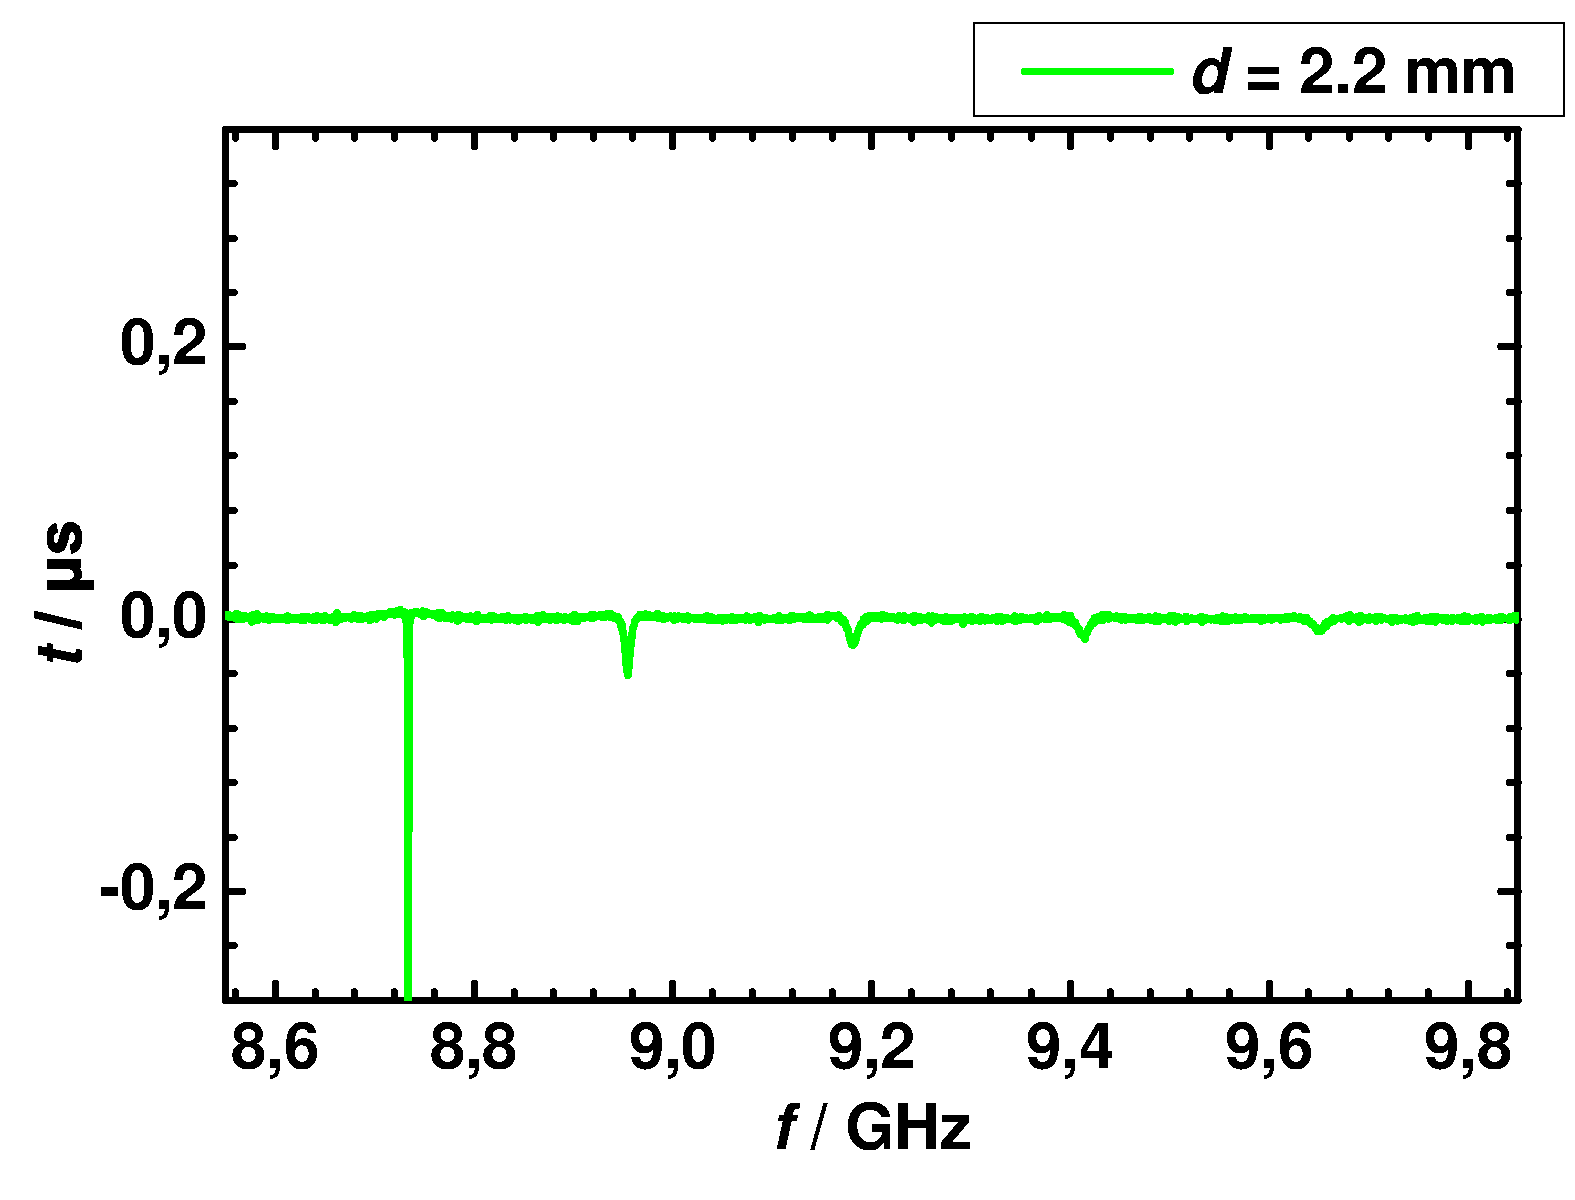
\includegraphics[totalheight=6 cm]{Grafiken/06_22.pdf} \label{fig:06_22}}
\caption{Group delay for different distances of the ring.}%
\label{fig:1_TE}%
\end{figure}
When moving the ring slowly away from the transmission line one can observe a change in time delay. At first, near the transmission line the transmission 

\chapter{Simulation}
In the next step a simulation with the program RSoft was performed. To reduce the computation time the 3D-structure was reduced to a 2D-structure using the effective index method. The simulation was performed in the optical frequency domain around 200~THz, so the dimensions of the waveguides had to be reduced by a factor of 20000. 

The strip waveguide with a length $l=5~\upmu$m was drawn in z-direction. For drawing the resonator rings two concentric cylinders with different diameters were created and subtracted from each other. The resulting index profile of the structure is shown in figure \ref{fig:index_profile1}.

In the first simulation a pulse was transmitted through the waveguide structure.



